\section{Definición de requisitos y análisis}
\label{sec:definicion_de_requisitos_y_analisis}

\subsection{Definición de requisitos}

A continuación se enumeran los requisitos para el desarrollo del trabajo:

\begin{itemize}
	\item Implementar y entrenar una red neuronal que genere un modelo capaz de detectar baches en el asfalto a partir de imágenes
	\item El modelo deberá ser capaz de procesar una imagen en un tiempo lo más cercano posible a 1/30s, para ser capaz de procesar video en tiempo real
	\item El modelo deberá poderse ejecutar en un dispositivo móvil Android
	\item El modelo será alimentado directamente con la salida de la cámara del dispositivo móvil
\end{itemize}

\subsection{Arquitectura}

\begin{figure}[H]
	\centering
	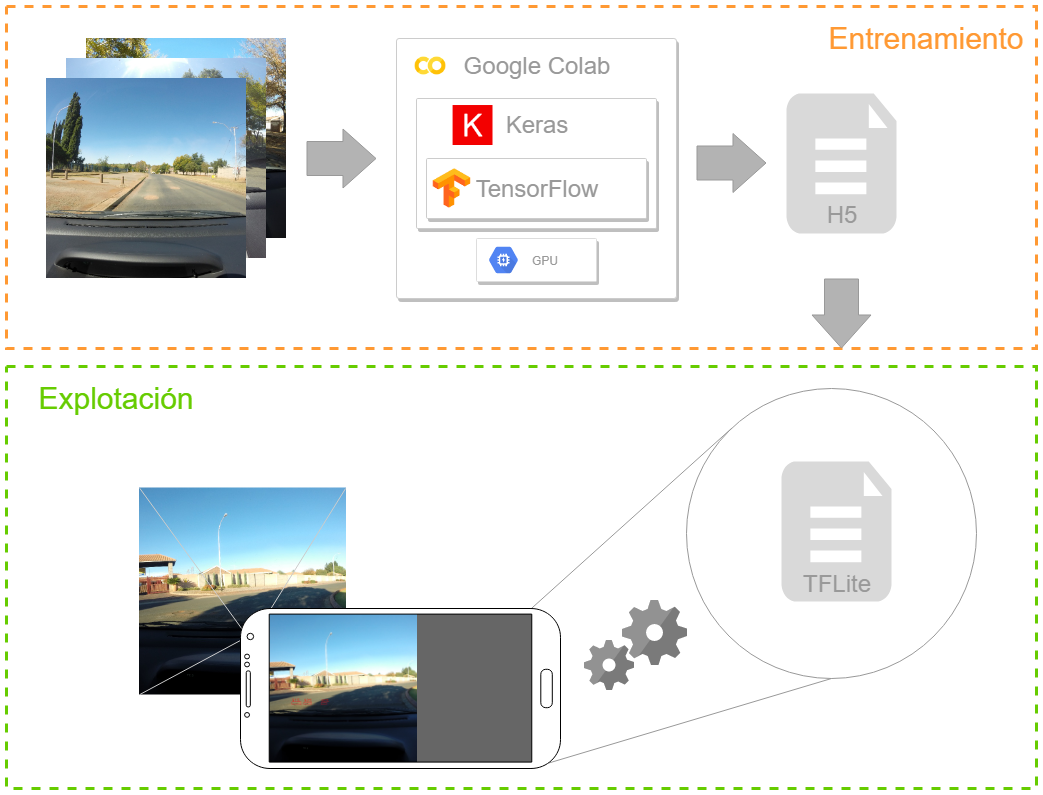
\includegraphics[width=\linewidth]{images/architecture.png}
	\caption{Arquitectura de la solución}
	\label{fig:architecture}
\end{figure}

Como se puede observar en la figura \ref{fig:architecture}, la arquitectura está dividida en dos partes. Una parte se utiliza para entrenar la red neuronal y generar el modelo. La otra parte se utiliza para explotar el modelo generado.

La parte utilizada durante el entrenamiento requiere de un hardware potente y del uso de GPU para reducir los tiempos de entrenamiento. La explotación del modelo, al contrario de lo que sucede con el entrenamiento, no requiere de un hardware potente y se ejecuta directamente en un dispositivo móvil en posesión del usuario final. El modelo obtenido después de la fase de entrenamiento, se transforma a un formato que está pensado para ser ejecutado en dispositivos con recursos limitados.

\subsection{Tecnologías}

Todo el proyecto ha sido desarrollado utilizando Python, salvo la aplicación Android, que ha sido desarrollada en Java.

Para el procesamiento de imágenes se ha utilizado el paquete Python OpenCV. Este procesamiento incluye la lectura de imágenes en formato jpg, recorte, reescalado y volteo de las imágenes, visualización de las predicciones obtenidas, etc.

Para la implementación de la red neuronal se ha utilizado Keras, que es un envoltorio sobre Tensorflow que simplifica su uso. Dada una arquitectura de red neuronal, con Keras es muy sencillo definir las capas y sus interconexiones. Además Keras proporciona clases que facilitan la definición de un conjunto de imágenes como entrada de la red neuronal. Keras también proporciona una serie de eventos con la idea de poder suscribirse a los mismos y poder reaccionar en consecuencia, como por ejemplo, suscribirse al evento de final de época y salvar el modelo si ha mejorado con respecto a la época anterior.

Las redes neuronales utilizadas en el proyecto no se han implementado de cero, sino que se ha partido de dos implementaciones en Keras de \textit{YOLO v3} \cite{s3_yolov3_orig} y \textit{YOLO v3 Tiny} \cite{s3_yolov3tiny_orig}. Se han unido ambas implementaciones en una única \cite{s3_yolo_dicastro} que soporta ambos tipos de red YOLO. También se han realizado múltiples desarrollos para mejorar la funcionalidad, como por ejemplo: soporte en formato txt de las etiquetas de las imágenes, nuevos parámetros de configuración para mejorar el resultado del entrenamiento, etc.

Para la ejecución de los modelos obtenidos en un dispositivo móvil de ha utilizado TFLite. Este paquete permite transformar distintos tipos de modelo (keras, tensorflow) a formato TFLite y ejecutar estos modelos en dispositivos con recursos reducidos. En las últimas versiones de esta librería se soporta, aunque de forma experimental, el uso de la GPU del dispositivo.

La aplicación móvil ha sido desarrollada en java para la plataforma Android. TFLite dispone de una librería java que simplifica la carga del modelo y su ejecución.